\documentclass[12pt,letterpaper]{scrartcl}
\usepackage{lipsum}
\usepackage[utf8]{inputenc}
\usepackage{amsmath}
\usepackage{amsfonts}
\usepackage{amssymb}
\usepackage{graphicx}
\usepackage[left=3cm,right=2.5cm,top=2.5cm,bottom=2.5cm]{geometry}
\usepackage[]{algorithm2e}
\author{Don cuyi}

%Color
\usepackage{color}
\definecolor{nred}{RGB}{174,49,54}
\definecolor{nblue}{RGB}{86,99,146}
\definecolor{nalgo}{RGB}{188,139,76}
\usepackage{sectsty}
\sectionfont{\color{nred}}
\subsectionfont{\color{nblue}}
\subsubsectionfont{\color{nalgo}}

%Librías tikz
\usepackage{pgf,tikz}
\usepackage{mathrsfs}
\usetikzlibrary{arrows}
\usetikzlibrary[patterns]
\newcommand{\degre}{\ensuremath{^\circ}}
\definecolor{qqwuqq}{rgb}{0.,0.39215686274509803,0.}
\definecolor{ffttww}{rgb}{1.,0.2,0.4}
%Hipervinculos
\usepackage{hyperref}

\usepackage{fancyhdr}
\pagestyle{fancy}
\fancyhead[L]{Combinatoria}
\fancyhead[C]{Licenciatura en ciencias de la computación}
\fancyhead[R]{USACH}

%interlineado
\renewcommand{\baselinestretch}{1.2}

%\bibitem{Yahoo} \textsc{Andres G} (2009),
%\textbf{¿Generar números aleatorios negativos en Lenguaje C?} En \textsc{Yahoo! respuestas}
%Recuperado el el 23 del julio del 2014
%\url{https://es.answers.yahoo.com/question/index?qid=20091121055249AAUQH3N}

\newcommand{\biblio}[7]{
\bibitem{#1} \textsc{#2} (#3),
\textbf{#4} En \textsc{#5}
Recuperado el #6
\url{#7}
}

% Last, F. M. (Year Published) Book. City, State: Publisher.
\newcommand{\book}[5]{
\bibitem{#1} \textsc{#2} (#3),
\textbf{#4}  \textsc{#5} Estado: Publicado
}

\begin{document}

\begin{titlepage}

\begin{center}

{\Large { Licenciatura en ciencia de la computación} }


\includegraphics[scale=1]{UDSCNRJ}
\\[1cm]

{\Huge \textsc{Algoritmo Euclideano}}\\[0.7cm]

{\huge  Matemática Computacional}\\[2cm]


\begin{minipage}[l]{0.4\textwidth}
	\begin{flushleft}
	\linespread{1}
		\textbf{\textsf{Profesor:}}\\
		\large Nicolas Thériault
	\end{flushleft}
\end{minipage}
\begin{minipage}[l]{0.4\textwidth}

	\begin{flushright}

		\textbf{\textsf{Autor:}}\\
		\linespread{1}
		\large Sergio Salinas\\
		\large Danilo Abellá\\

	\end{flushright}
\end{minipage}

\end{center}

\end{titlepage}



\newpage
\section*{Introducción}


\section{Tiempos de ejecución de Algoritmo}

A continuación se mostrarán los tiempos de ejecución apra cada valor de "n" y "p" respectivamente.

\subsection{Tiempos de ejecución para valores de "n" y "p".}

Costos computacionales de los algoritmos donde: \[p \in \{1/10, 3/10, 1/2, 7/10, 9/10\} \] para distintos valores de n:
\\\\
n=18
\\\\
	p=0.1\hspace{1cm}57.0000000
\\
	p=0.3\hspace{1cm}43.0000000
\\
	p=0.5\hspace{1cm}41.0000000
\\
	p=0.7\hspace{1cm}128.0000000
\\
	p=0.9\hspace{1cm}40.0000000
\\\\
n=660
\\\\
	p=0.1\hspace{1cm}18815.0000000
\\
	p=0.3\hspace{1cm}18698.0000000
\\
	p=0.5\hspace{1cm}26974.0000000
\\
	p=0.7\hspace{1cm}18506.0000000
\\
	p=0.9\hspace{1cm}21156.0000000
\\\\
n=8000
\\\\
	p=0.1\hspace{1cm}2890310.0000000
\\
	p=0.3\hspace{1cm}3851808.0000000
\\
	p=0.5\hspace{1cm}5042122.0000000
\\
	p=0.7\hspace{1cm}6085456.0000000
\\
	p=0.9\hspace{1cm}6920520.0000000
\\\\
\subsection{Costo computacional para n = 1000.}

Costos computacionales de los algoritmos para n = 1000 para distintos valores de p.
\\
Tiempos de espera para los siguientes valores de "p":
\\\\
	p=0\hspace{1cm}34094.0000000
\\
	p=0.1\hspace{1cm}31610.0000000
\\
	p=0.2\hspace{1cm}37190.0000000
\\
	p=0.3\hspace{1cm}55043.0000000
\\
	p=0.4\hspace{1cm}47476.0000000
\\
	p=0.5\hspace{1cm}45258.0000000
\\
	p=0.6\hspace{1cm}46934.0000000
\\
	p=0.7\hspace{1cm}56155.0000000
\\
	p=0.8\hspace{1cm}56874.0000000
\\
	p=0.9\hspace{1cm}47229.0000000
\\
	p=1\hspace{1cm}48239.0000000


\newpage
\section{Formulación experimentos}

\section{Información de Hardware y Software}


\subsection{ Notebook - Danilo Abellá}
\subsubsection{Software}
\begin{itemize}
\item SO: Xubuntu 16.04.1 LTS
\item GMP Library
\item Mousepad 0.4.0
\end{itemize}

\subsubsection{Hardware}
\begin{itemize}
\item AMD Turion(tm) X2 Dual-Core Mobile RM-72 2.10GHz
\item Memoria (RAM): 4,00 GB(3,75 GB utilizable)
\item Adaptador de pantalla: ATI Raedon HD 3200 Graphics
\end{itemize}



\subsection{Notebook - Sergio Salinas}
\subsubsection{Software}
\begin{itemize}
\item  SO: ubuntu Gnome 16.04 LTS
\item Compilador: gcc version 5.4.0 20160609 
\item Editor de text: Atom
\end{itemize}

\subsubsection{Hardware}
\begin{itemize}
\item Procesador: Intel Core i7-6500U CPU  2.50GHz x 4 
\item Video: Intel HD Graphics 520 (Skylake GT2) 
\end{itemize}


\newpage

\section{Curvas de desempeño de resultados}
\subsection{Comportamiento para los valores de "p" pedidos.}

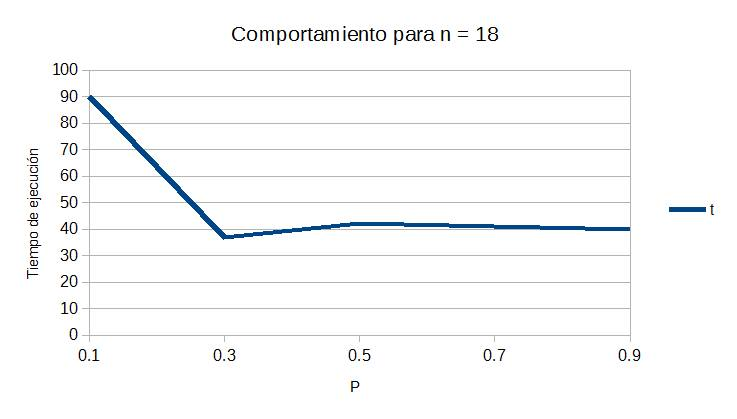
\includegraphics[scale=0.55]{n}

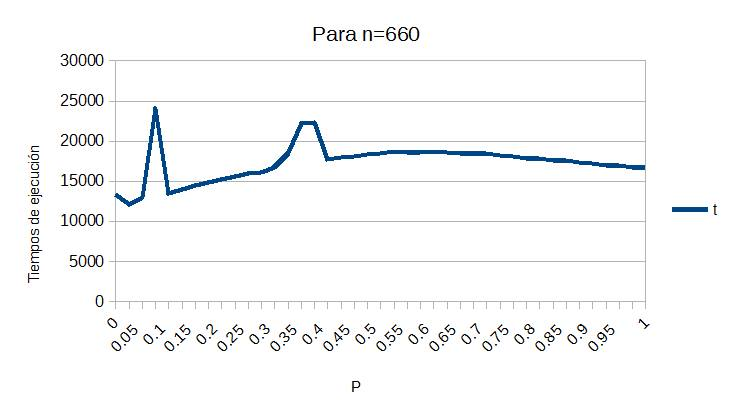
\includegraphics[scale=0.55]{nn}

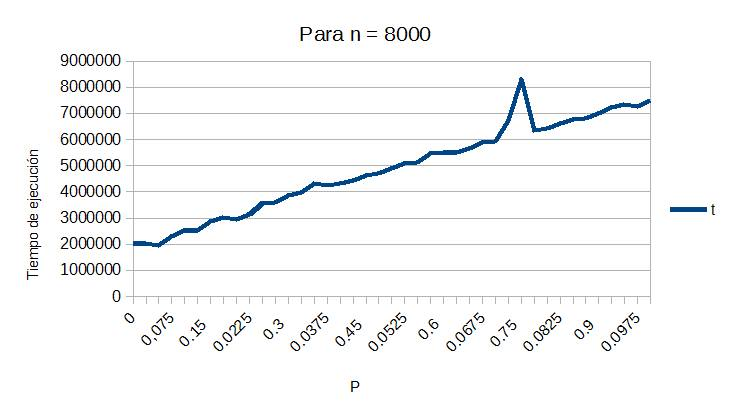
\includegraphics[scale=0.55]{nnnn}

\subsection{Costos computacionales de los algoritmos para n = 1000 para distintos valores de "p".}

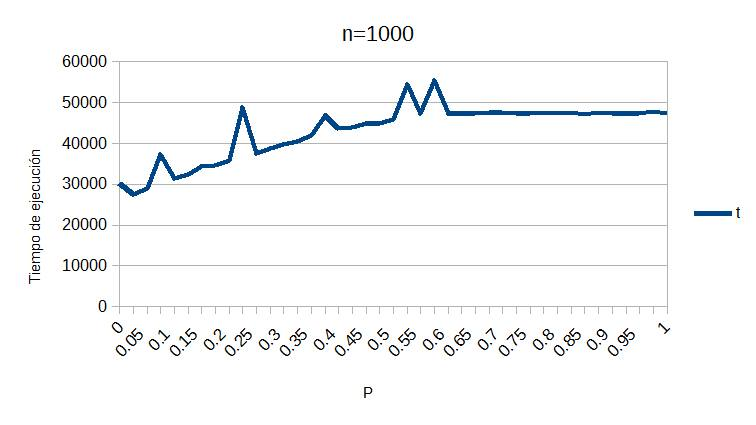
\includegraphics[scale=0.55]{nnn}

\newpage
\section{Conclusiones}

\end{document}